\documentclass[]{article}
\usepackage{lmodern}
\usepackage{amssymb,amsmath}
\usepackage{graphicx}
\usepackage{hyperref}
\hypersetup{pdfborder={0 0 0}, breaklinks=true}

\makeatletter
\def\fps@figure{htbp}
\makeatother

\title{CS4102 Practical 2}
\author{140015533}
\date{27 April 2018}

\begin{document}
\maketitle

\section{Introduction}

In this practical I implement a simple program for rendering a 3D model of a face. The model is defined as a collection of triangles, with the vertices of each triangle specified. The model also has a texture, defined as a greyscale value at each vertex of each triangle.

Orthographic projection and flat shading is used to render the face. Lambert's illumination model is used for calculating the intensity of each triangle and the light position and intensity is configurable by the user. The texture is mapped using simple interpolation.

\section{Design and Implementation}

\subsection{Data Structures}

Information about each triangle is stored in the \texttt{Triangle} class, which contains two matrices.

The first one is a position. The three vertex vectors are stored in one matrix, therefore the size of the matrix is $3 \times 3$. The first column contains the first vertex, the second column the second vertex and so on. The texture information is stored in another matrix, which has one column and three rows. Each colour value is stored on one row.

I used matrices to store the information to reduce the number of fields in the \texttt{Triangle} class and possibly to allow some matrix operations to be done on the values.

The \texttt{Triangle} class has two methods: for calculating the centeroid and the surface normal vector. The centeroid is obtained by simply multiplying all three vertices by $\frac{1}{3}$ and adding them. The surface normal is calculated as the cross product of two sides of the triangle: $(p_2 - p_1) \times (p_3 - p_1)$.

\subsection{Parsing}

The \texttt{Parser} class is responsible for reading the input files and generating a list of triangles. It uses the \texttt{Scanner} library class to parse numbers from the files. Both files are read simultaneously.

The texture data file contained some odd values -- for example, on line 58101 there is a negative value. I chose to ignore these values and use 0 instead, as it does not make sense for the colour value to be negative.

\subsection{Camera}

Since we do not have 3D screens, the 3D coordinates of the triangles need to be projected onto a 2D canvas that can be displayed to the user. I used a simple orthographic projection, where the z-coordinate can be simply removed if the camera is pointing along the z-axis.

The projection alone is not enough though. The vertex coordinates are too large to fit on the screen, therefore they need to be scaled down. To achieve this, I defined a window which the camera should cover, for example $240000 \times 160000$ units, and the canvas size, for example $1200 \times 800$ pixels. To get the scaling factor, I simply calculate the ratio of screen size and window size. In this case it is $0.005$ for both directions.

Since the model is arranged roughly around the $[0, 0, 0]$ point, it needs to be translated as well, otherwise only a quarter of the face would be visible, as the canvas renders the origin in one of the corners. The model is translated by a half of the window size, so that it is in the middle of the projection.

Finally, the projection needs to be mirrored around the x-axis. This is simply because the canvas renders the origin in the top left corner, with the y-axis pointing down, but the model assumes that the y-axis is pointing up.

If we use homogeneous coordinates for the vertices, we can derive a single matrix that will apply all of these transformations, as shown below. $t_x$ and $t_y$ are the values for translation, $s_x$ and $s_y$ are scaling factors. The matrices are (in the order shown) the scaling, translation, mirroring and orthographic projection.

\[
  \begin{bmatrix}
    s_x & 0 & 0 \\
    0 & s_y & 0 \\
    0 & 0 & 1
  \end{bmatrix}
  %
  \begin{bmatrix}
    1 & 0 & t_x \\
    0 & 1 & t_y \\
    0 & 0 & 0
  \end{bmatrix}
  %
  \begin{bmatrix}
    1 & 0 & 0 \\
    0 & -1 & 0 \\
    0 & 0 & 1
  \end{bmatrix}
  %
  \begin{bmatrix}
    1 & 0 & 0 & 0 \\
    0 & 1 & 0 & 0 \\
    0 & 0 & 0 & 1
  \end{bmatrix}
  =
  \begin{bmatrix}
    s_x & 0 & 0 & s_x t_x \\
    0 & s_y & 0 & s_y t_y \\
    0 & 0 & 0 & 1
  \end{bmatrix}
\]

The final matrix is used by the camera to project 3D coordinates into 2D space. Since the rest of the program is not using homogeneous coordinates, the input first needs to be homogenised and then de-homogenised.

\subsection{Illumination}

Illumination is implemented in the \texttt{Light} class. It has two attributes, position (a 3D vector) and intensity (value from 0 to 1). The class has a method for calculating the illumination intensity for a specific point. The position of the point and the surface normal need to be specified.

Lambert's illumination model is used to calculate the intensity for each point, with the diffusion coefficient set to 1 and the intensity specified by the attribute.

\subsection{Rendering}

The \texttt{Renderer} class handles all logic related to rendering the triangles on a 2D canvas. It uses the \texttt{Light} and \texttt{Camera} classes to calculate the illumination and project 3D coordinates.

Before the triangles can be rendered, they need to be sorted so that the triangles most distant from the camera are render first -- this is essentially the painter's algorithm. Since I am using orthographic projection and the camera is pointed in line with the z-axis, the triangles are simply sorted by the z-coordinate of their centeroids.

Once triangles are sorted, they can be rendered to the canvas. The 3D vertices of each triangle are first projected to the 2D coordinate system of the canvas. The illuminance is calculated from the triangle centeroid and the surface normal vector. The illuminance value is used to multiply the texture matrix, so that the colours are less prominent if the triangle is not illuminated properly.

To draw a single triangle on the canvas, all pixels contained in the triangle need to be filled with the correct colour based on the texture.

I chose to use a simple algorithm for filling the triangle. It essentially interpolates between the three vertices and colours. This is done by defining two variables, $j$ and $k$ such that $j, k \in [0, 1]$ and $j + k \leq 1$. A third variable, $i$, is based on $j$ and $k$: $i = 1 - j - k$. Therefore, it is always true that $i + j + k = 1$.

These three variables are used to multiply the vertex points and the colour values. For example, to get the position and colour of a point in the middle of the triangle, we set $i = j = k = \frac{1}{3}$. The position of the point is then $p = i a + j b + k c$, where $a$, $b$ and $c$ are vertices of the triangle. The colour is calculated similarly, by multiplying each of the three values by the corresponding variable.

The exact values of $j$ and $k$ are calculated by sampling the range $[0, 1]$. The number of samples depends on the size of the projected triangle. The bounding box for the triangle is calculated and either the width or height (the higher value is selected) is used as the sample size. So, for example, if the bounding box is 3 pixels wide and 2 pixels tall, there are 3 samples, so values of $j$ and $k$ are 0, 0.5 and 1. This way all pixels in the triangle are covered.

One problem is that the sampled positions are not integers, but since pixel positions need to be integers, the samples are simply rounded up or down.

\subsection{User Interface}

The user interface is implemented using JavaFX. There is a single canvas for rendering the image, and a number of text inputs and a button for controlling the light position and intensity.

Most of the UI logic is contained in the \texttt{Controller} class, which simply reads the values from the inputs and uses \texttt{Rendered} to render the image.

The user interface is shown in Figure \ref{fig:ui}.

\begin{figure}
  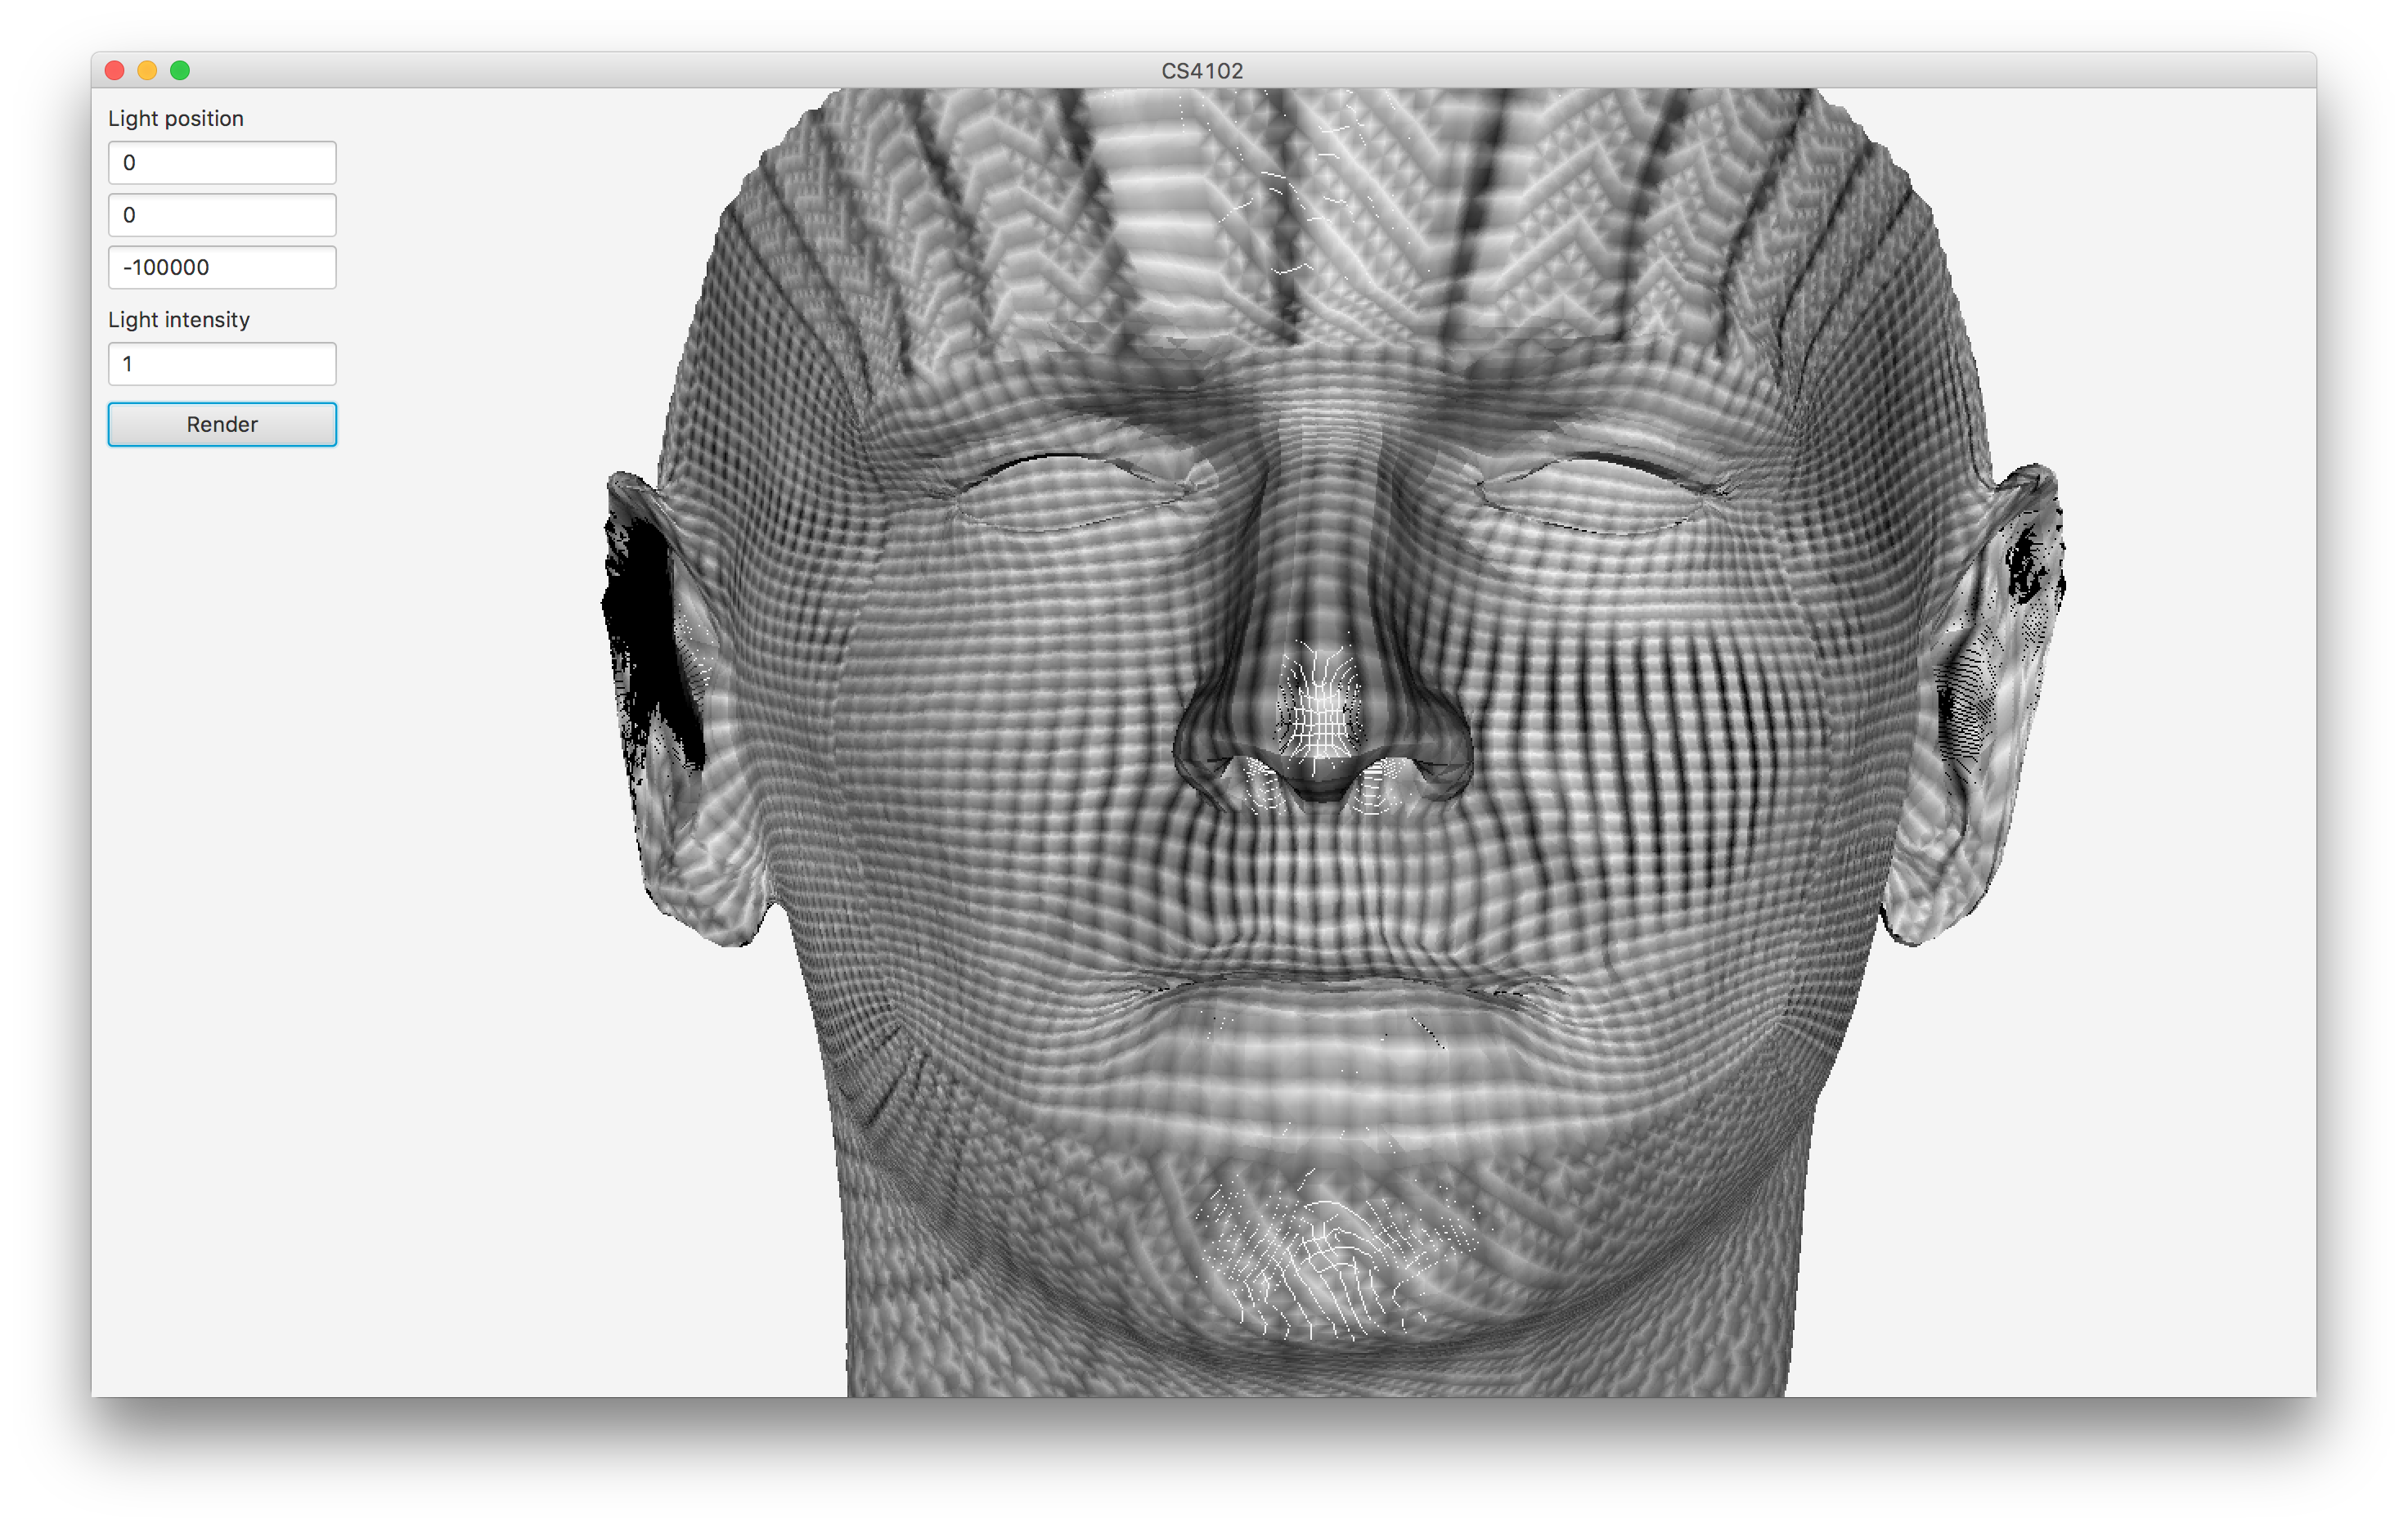
\includegraphics[width=\textwidth]{figures/ui}
  \caption{Screenshot of the user interface}
  \label{fig:ui}
\end{figure}

\section{Testing}

There are some unit tests that I used to make sure that the calculation of the camera transform matrix and homogenising and de-homogenising coordinates work correctly.

I tested the program manually. At first I defined a simple model that contained only a few triangles, to see if the projection and rendering onto the canvas is working correctly. Once I had this implemented, I used the supplied face model to test the translation and scaling in the camera, and to see if rendering of triangles is working correctly.

I used a simple model again when I was implementing texture mapping, to see if the colour interpolation is working correctly. This model can be seen in Figure \ref{fig:triangle}.

\begin{figure}
  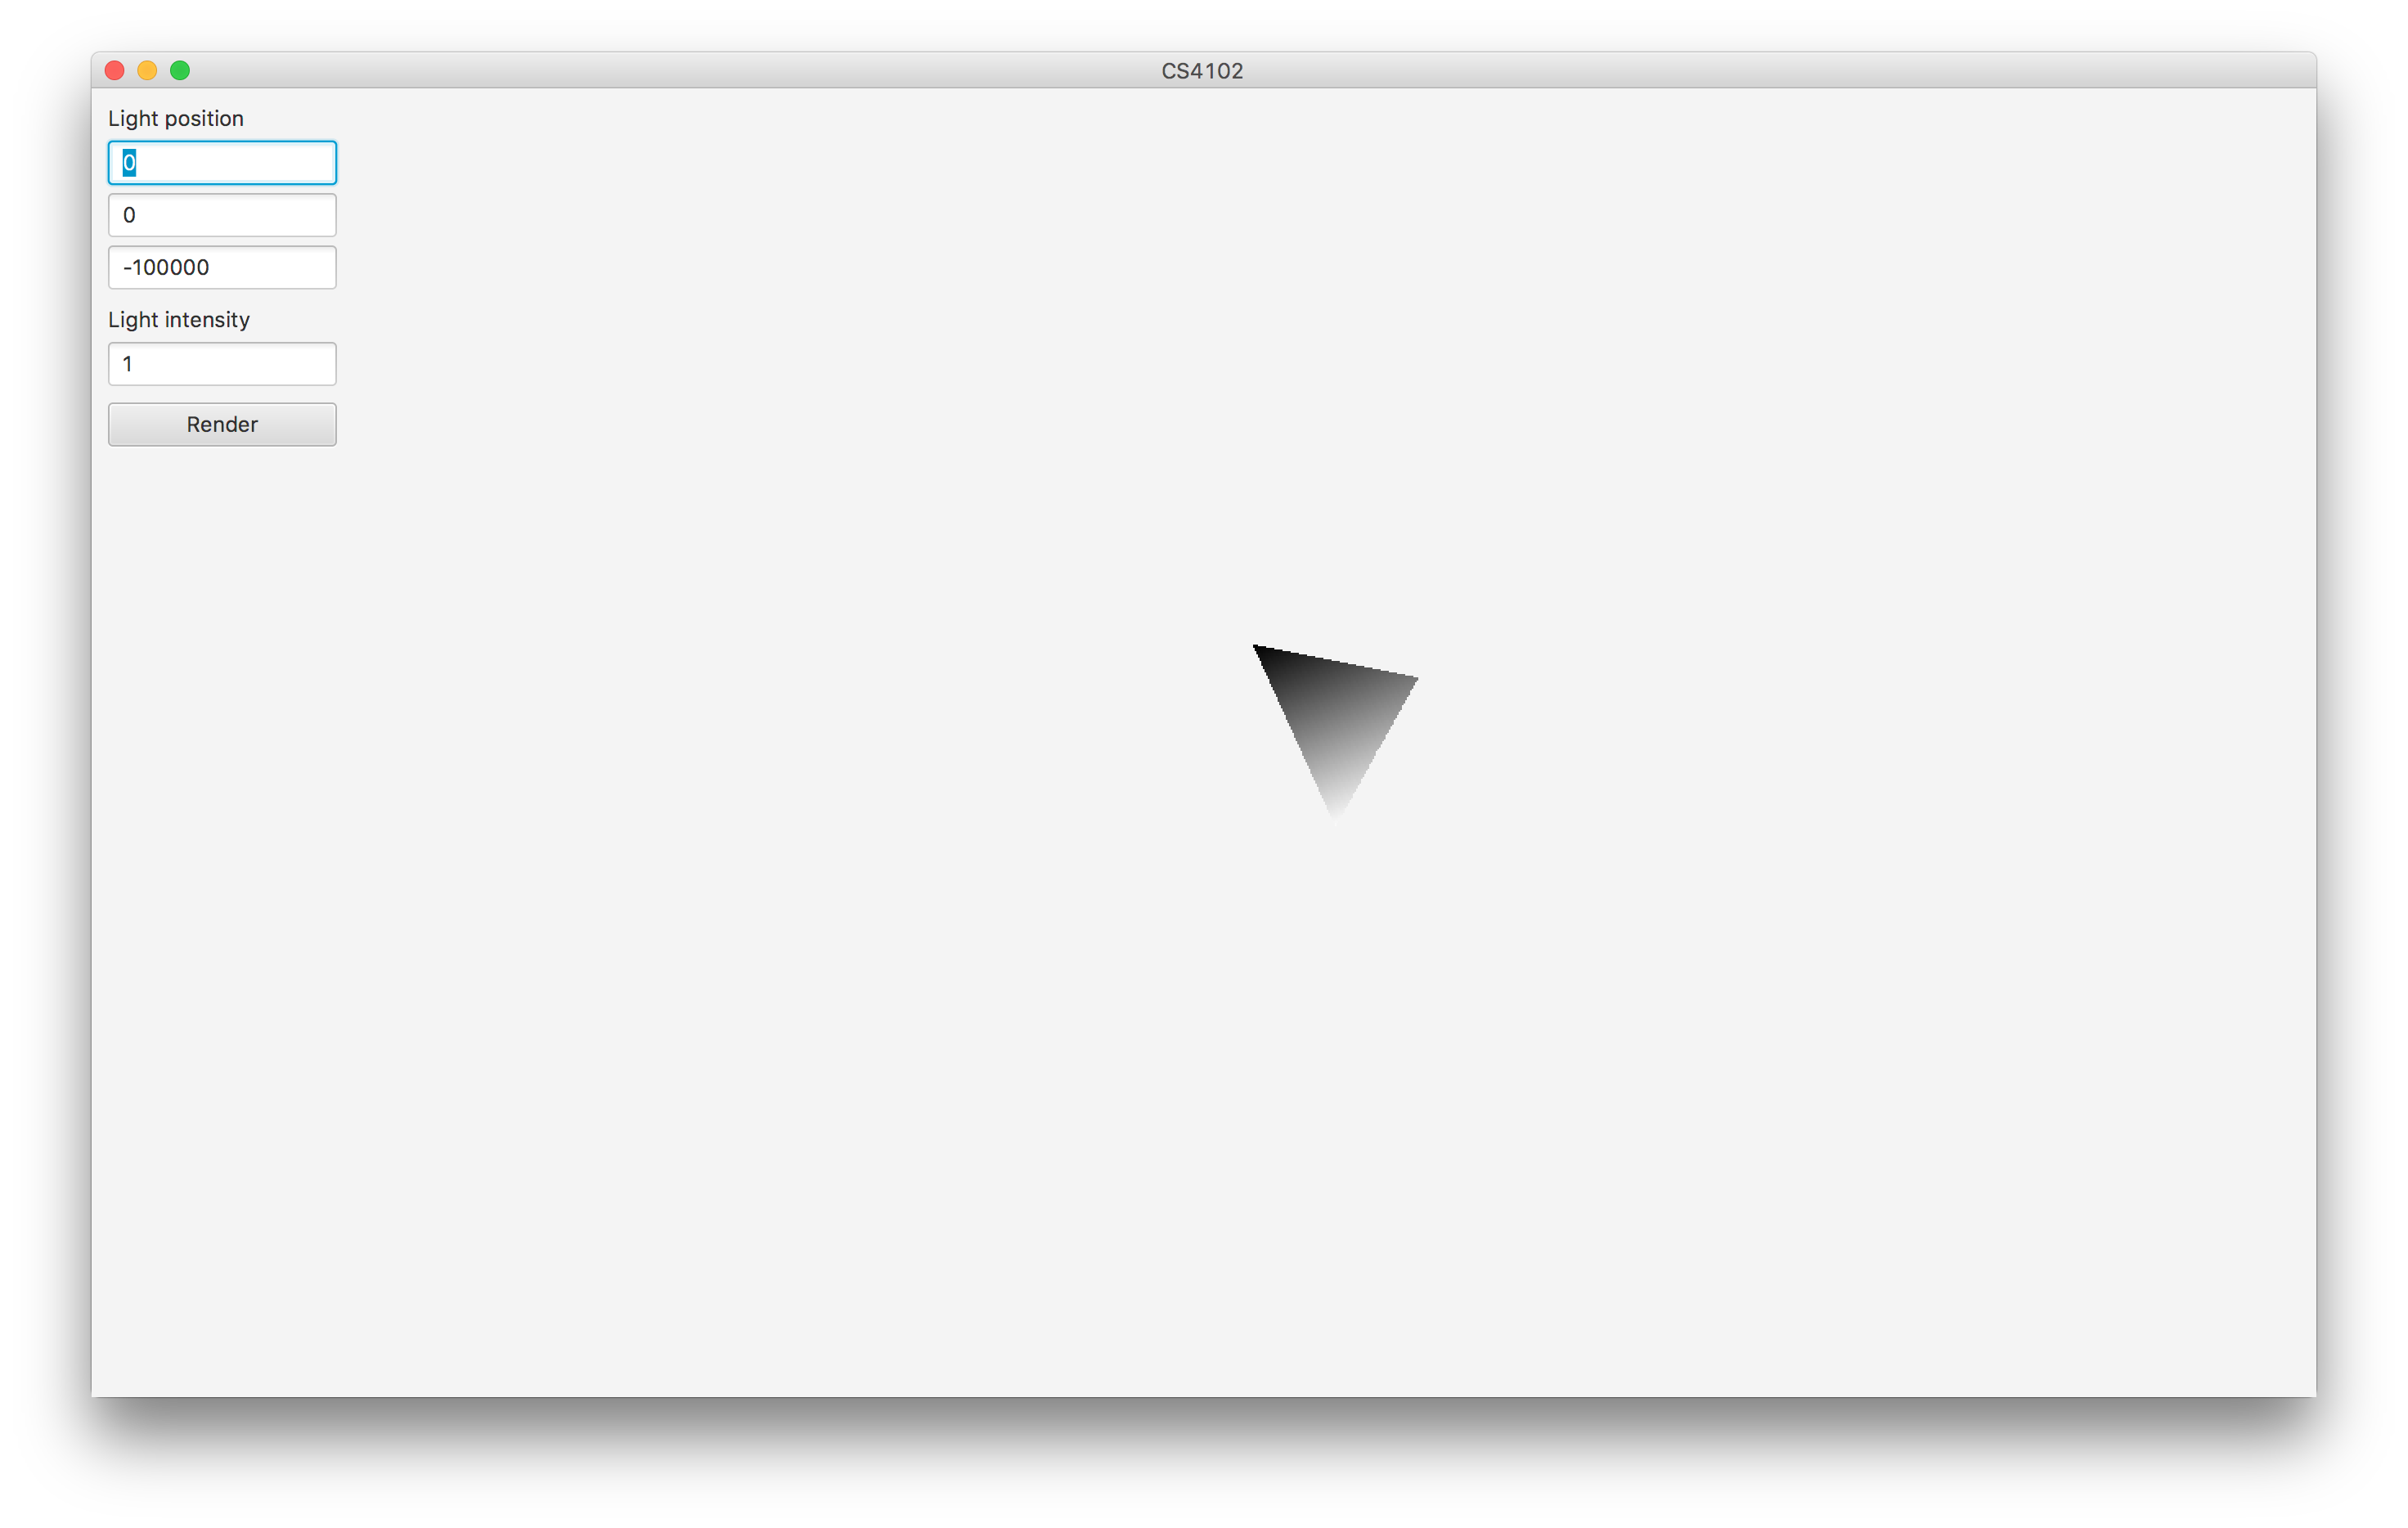
\includegraphics[width=\textwidth]{figures/triangle}
  \caption{Testing model}
  \label{fig:triangle}
\end{figure}

Since there is no reference image for the result, I tried to examine the rendered image, look for odd features and compare them with the input files.

\section{Evaluation}

I completed the basic specification. The application renders the model of a face using flat shading, orthographic projection and Lambert's illumination model. User can configure the position and the intensity of the light source. The supplied texture is applied by interpolating the three colours on the triangle. The final version of the application with configured light position can be seen in Figure \ref{fig:illuminated}.

\begin{figure}
  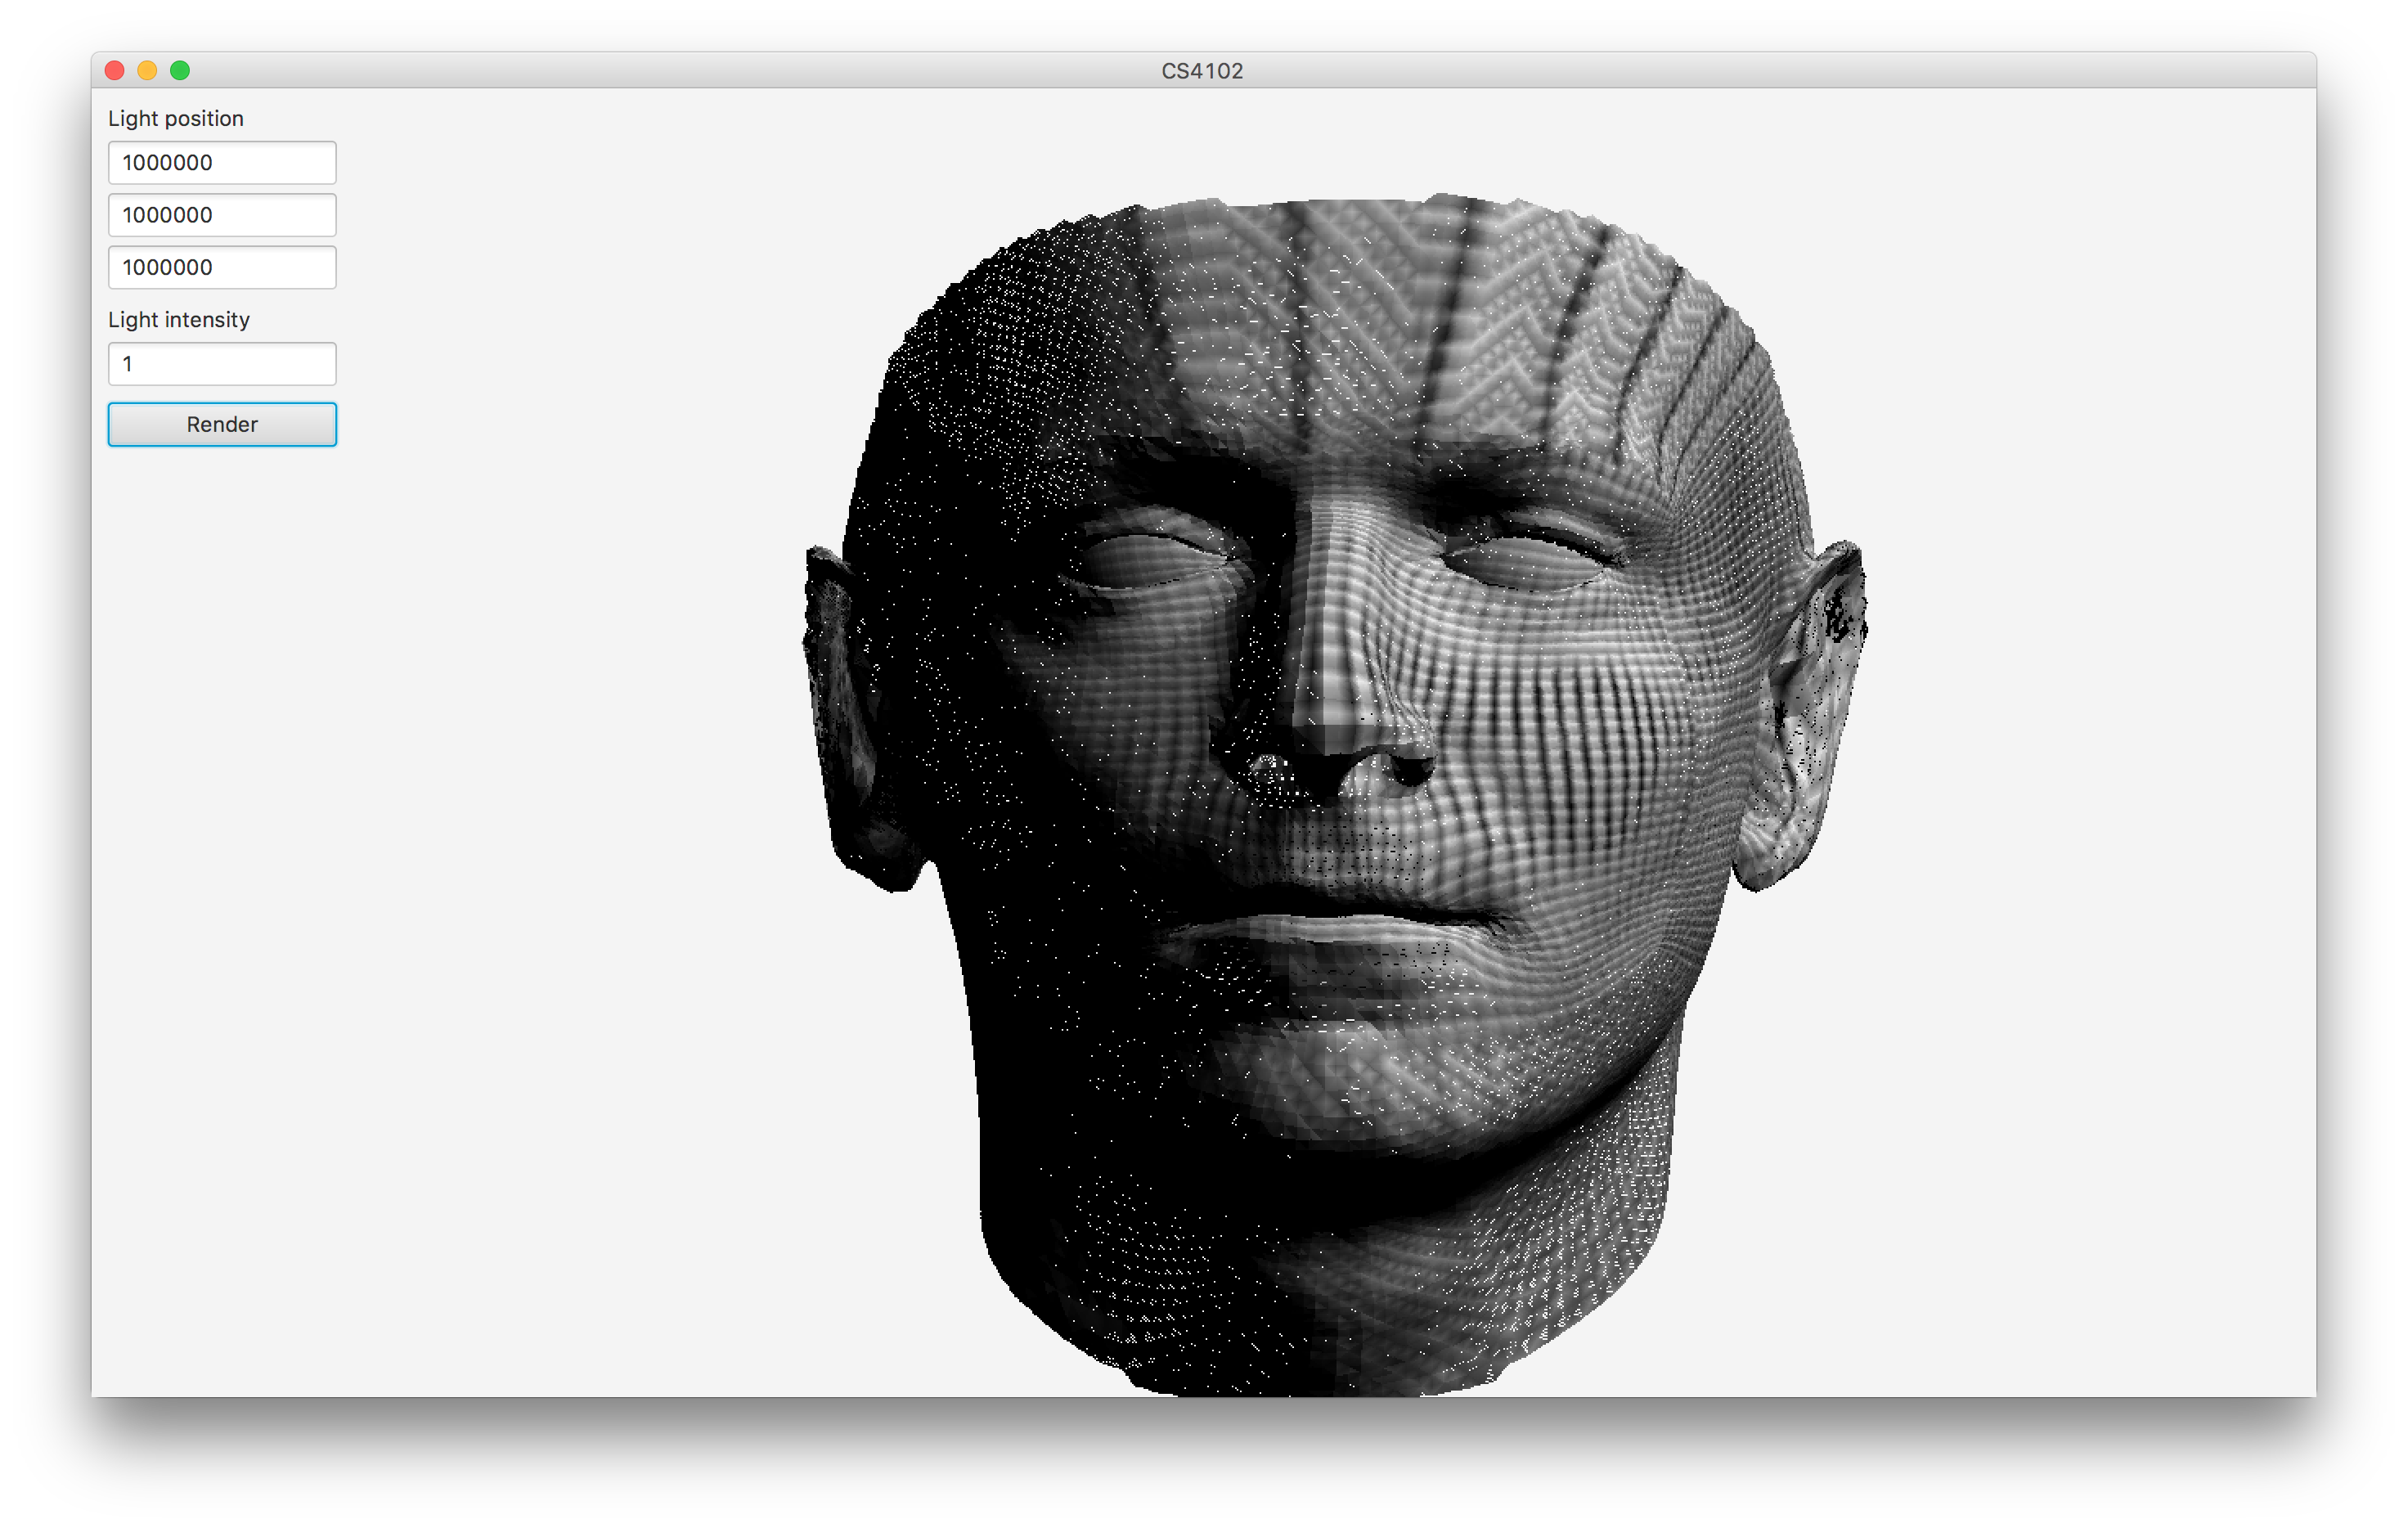
\includegraphics[width=\textwidth]{figures/illuminated}
  \caption{Application with the illuminated model}
  \label{fig:illuminated}
\end{figure}

However, my implementation has some drawbacks. The rendering process is quite slow and there are definitely possibilities for optimisation. For instance, z-buffering and back-face culling could be used to reduce the number of rendered triangles.

The camera is fixed to point in line with the z-axis. A more realistic panoramic projection could be used instead of orthographic.

There are some visual artefacts between the triangles. This is due to the triangle fill algorithm, as it is not precise and there might be gaps between edges of adjacent triangles. No anti-aliasing is implemented, so the edges of diagonal lines are not smooth.

\section{Conclusion}

My task in this practical was to create a program that would render a 3D model, defined in two input files containing the positions of vertices and the colours for each vertex. Simple techniques and algorithms are used to render the model, however the result is a fairly realistic image.

This was an interesting exercise in simple computer graphics processes and algorithms. I was able to apply the knowledge gained from this module to a real application and see what it takes to render a 3D model.

\end{document}
